\documentclass[10pt,a4paper]{article}
\usepackage{amsmath}
\usepackage{amssymb}
\usepackage{graphicx}
\usepackage{color}
\usepackage{fancyhdr}
\usepackage{fancyvrb}
\usepackage[margin=3.5cm]{geometry}
\usepackage{framed}
\usepackage{enumerate}
\usepackage{textcomp}
\def\ket#1{\left|#1\right\rangle}
\def\bra#1{\left\langle#1\right|}
\def\braket#1{\left\langle#1\right\rangle}

\definecolor{linkcol}{rgb}{0.0, 0.0, 0.7}
\usepackage[colorlinks=true,urlcolor=linkcol,citecolor=black,linkcolor=linkcol]{hyperref}

\setcounter{section}{3}
\renewcommand\thesection{\arabic{section}}
\renewcommand\thesubsection{\thesection.\arabic{subsection}}

\fancyhf{}
\lhead{\tiny Y.~D.~Chong (2020)}
\rhead{\scriptsize MH2801: Complex Methods for the Sciences}
\lfoot{}
\rfoot{\thepage}
\pagestyle{fancy}

\begin{document}
\setcounter{page}{30}

\section{Complex Oscillations}
\label{complex-oscillations}

In physics and the other quantitative sciences, complex numbers are
widely used for analyzing oscillations and waves. We begin our study
of this topic with an important elementary model called the
\textbf{damped harmonic oscillator}.

\subsection{The damped harmonic oscillator}
\label{the-damped-harmonic-oscillator}

Consider a particle of mass $m$ subject to a spring force and a
damping force. The particle can move along one dimension, with $x(t)$
denoting its displacement at time $t$. The damping coefficient is $2m
\gamma$, and the spring constant is $k = m\omega_0^2$. The parameters
$m$, $\gamma$, and $\omega_0$ are all positive real numbers.

\begin{figure}[ht]
  \centering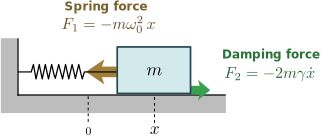
\includegraphics[width=0.55\textwidth]{oscillator}
\end{figure}

The motion of the particle can be derived using Newton's second law:
\begin{equation}
  m \frac{d^2 x}{dt^2} = F(x,t) = - 2m\gamma \frac{dx}{dt} - m\omega_0^2 x(t).
\end{equation}
Dividing by the common factor of $m$, and bringing everything to one
side, gives
\begin{equation}
  \frac{d^2 x}{dt^2} + 2\gamma \frac{dx}{dt} + \omega_0^2 x(t) = 0.
\end{equation}
This is called the \textbf{damped harmonic oscillator equation}.

\begin{framed}\noindent
  \textit{Note}---Sometimes, we write the damped harmonic oscillator
  equation as:
  \begin{equation}
    \left[\frac{d^2}{dt^2} + 2\gamma \frac{d}{dt} + \omega_0^2 \right]\, x(t) = 0.
  \end{equation}
  The quantity in square brackets is a linear differential operator
  acting on $x(t)$. The three terms in the operator correspond to the
  three ``ingredients'' of the damped harmonic oscillator model: (i) a
  second derivative term stemming from Newton's second law, (ii) a
  first derivative term representing the effects of damping, and (iii)
  a constant term representing the oscillation induced by the spring
  force.

  Writing the equation this way helps emphasize that it is linear:
  i.e., any superposition of solutions is likewise a solution (see
  Section~\ref{complex-ansatz}).
\end{framed}

\subsubsection{Behavior of the solution}
\label{behavior-of-the-solution}

The damped harmonic oscillator equation is a second-order ordinary
differential equation (ODE).  Its general solution must contain two
free parameters, which are usually (but not necessarily) specified by
the initial displacement $x(0)$ and initial velocity $\dot{x}(0)$.

For $\gamma = 0$ (zero damping), the system reduces to the
\textbf{simple harmonic oscillator}. From previous physics courses, we
know that the general solution to the simple harmonic oscillator has
the form
\begin{equation}
  x(t) = A \cos(\omega_0 t + \phi),
  \label{simple-gensol}
\end{equation}
where $A$ and $\phi$ are free parameters. This describes a sinusoidal
motion with constant amplitude $A$, phase $\phi$, and frequency
$\omega_0$.

By the way, some authors call $\omega_0$ an ``angular frequency'',
reserving the term ``frequency'' for the quantity $f_0 =
\omega_0/2\pi$. But we will always deal with $\omega_0$ rather than
$f_0$. As such, we can refer to $\omega_0$ as ``frequency'' for
brevity, without risk of ambiguity.

The quantity $\omega_0$ is directly related to the spring constant by
$k = m\omega_0^2$; in fact, this is precisely why we parameterized the
spring constant in this way. It is called the \textbf{natural
  frequency} --- i.e., the natural oscillation frequency of the system
when damping is absent.

Eq.~\eqref{simple-gensol} can be re-expressed in terms of the initial
displacement $x(0) = x_0$ and initial velocity $\dot{x}(0) = v_0$. It
is straightforward to show that
\begin{equation}
  A = \sqrt{x_0^2 + \left(\frac{v_0}{\omega_0}\right)^2},
  \quad \phi = -\tan^{-1}\left(\frac{v_0}{\omega_0 x_0}\right).
\end{equation}

Now consider $\gamma > 0$. A damping force now opposes the motion,
doing work against the particle and causing it to lose energy over
time.  Hence, the particle can no longer oscillate forever around the
equilibrium position. If the damping force is relatively weak, the
energy lost per cycle is relatively small, so the motion of the
particle should consist of an oscillation whose amplitude diminishes
slowly over time. For $t \rightarrow \infty$, both $x$ and $\dot{x}$
go to zero.
        
\subsection{Complex solution}
\label{complex-solution}

The variable $x(t)$ is the displacement of the particle, so it ought
to be real. However, a good way to solve the damped harmonic
oscillator equation is to generalize $x(t)$ to \emph{complex} values.
In other words, we convert the harmonic oscillator equation into a
complex ODE:
\begin{equation}
  \frac{d^2 z}{dt^2} + 2\gamma \frac{dz}{dt} + \omega_0^2 z(t) = 0,
  \quad z(t) \in \mathbb{C}.
\end{equation}
The parameter-counting rule for real ODEs (see Chapter 1) generalizes
to complex ODEs, but the parameters are now complex numbers. As the
complex damped harmonic oscillator equation is a second-order ODE, its
general solution must have two complex free parameters.

Let us now figure out how to obtain the general solution to the
complex damped harmonic oscillator equation.  Then we will see how to
use it to solve the real problem.

\subsubsection{Complex ansatz}
\label{complex-ansatz}

To derive the general solution, first note that the damped harmonic
oscillator equation is linear. If we have two solutions $z_1(t)$ and
$z_2(t)$, then any superposition
\begin{equation}
  \psi_1 \, z_1(t) + \psi_2 \,z_2(t),\quad \mathrm{where}\;\, \psi_1, \psi_2 \in \mathbb{C}
\end{equation}
is also a solution. This can be verified by direct substitution into the
ODE.

Therefore, a good strategy for obtaining the general solution is to find
two specific solutions and superpose them. The two coefficients,
$\psi_1$ and $\psi_2$, would then serve as the general solution's
two free parameters.

We can make a guess (or an \textbf{ansatz}) for a specific solution:
\begin{equation}
z(t) = e^{-i\omega t}.
\end{equation}
Here, $\omega$ is a constant to be determined (which could be
complex). The first and second derivatives are:
\begin{align}
  \frac{dz}{dt} &= -i\omega\, e^{-i\omega t} \\
  \frac{d^2z}{dt^2} &= -\omega^2\, e^{-i\omega t}
\end{align}
Substituting these into the differential equation gives:
\begin{equation}
  \left[-\omega^2 - 2i\gamma \omega + \omega_0^2 \right] e^{-i\omega t} = 0.
\end{equation}
This equation holds for all $t$ if and only if the complex
second-order polynomial on the left-hand side is zero:
\begin{equation}
  -\omega^2 - 2i\gamma \omega + \omega_0^2 = 0.
\end{equation}
The solutions for $\omega$ can be obtained from the quadratic formula:
\begin{equation}
  \omega = -i\gamma \pm \sqrt{\omega_0^2 - \gamma^2}.
\end{equation}
Hence, we have found specific solutions that involve \emph{complex}
frequencies:
\begin{equation}
  z(t) = \exp\big(-i\omega_\pm t\big), \;\;\mathrm{where}\;\;
  \omega_\pm = -i\gamma \pm \sqrt{\omega_0^2 - \gamma^2}.
\end{equation}
For each value of $\gamma$ and $\omega_0$, both $\omega_+$ and
$\omega_-$ yield valid specific solutions.

\subsubsection{Complex frequencies}
\label{complex-frequencies}

What does it mean to have an oscillation with a complex frequency? If
we write the real and imaginary parts of the frequency as $\omega =
\omega_R + i \omega_I$, then
\begin{equation}
z(t) = e^{-i\omega t} = e^{\omega_I t} \; e^{-i\omega_R t}.
\end{equation}

If both $\omega_R$ and $\omega_I$ are non-zero, this describes a
spiral trajectory in the complex plane whose magnitude either
increases or decreases with time, depending on the sign of
$\omega_I$. To see this explicitly, we can write
\begin{equation}
z(t) = e^{\omega_I t} \; e^{-i\omega_R t} = R(t)\, e^{i\theta(t)}, \;\;\mathrm{where}\;\,\begin{cases}\displaystyle R(t) &= e^{\omega_I t}, \\ \displaystyle \theta(t) &= -\omega_R t.\end{cases}
\end{equation}
The real part of $\omega$ determines the oscillation frequency, and
the imaginary part determines whether the amplitude grows with time
(amplification) or shrinks with time (damping). A positive imaginary
part implies amplification, and a negative imaginary part implies
damping; zero imaginary part (i.e., a real frequency) implies
constant-amplitude oscillation.

Now let's look at the complex frequencies appearing in the specific
solutions to the damped harmonic oscillator:
\begin{equation}
\omega_\pm = -i\gamma \pm \sqrt{\omega_0^2 - \gamma^2}.
\end{equation}
In the plot below, you can see how the position of $\omega_\pm$ in the
complex plane depends on the values of $\gamma$ and $\omega_0$:

\begin{figure}[ht]
  \centering\includegraphics[width=0.76\textwidth]{oscillator_frequencies}
\end{figure}

\clearpage
In particular, note the following features:

\begin{itemize}
\item
  For $\gamma = 0$ (zero damping), the two frequencies are both real,
  and take the values $\pm \omega_0$. This corresponds to simple
  harmonic oscillation at the oscillator's natural frequency.
\item
  If we increase $\gamma$ from zero with $\omega_0$ fixed, both
  $\omega_+$ and $\omega_-$ move downwards in the complex plane,
  along a circular arc. Since the imaginary part of the frequencies are
  negative, the particle undergoes damped oscillation. This is called
  \textbf{under-damped motion}.
\item
  At $\gamma = \omega_0$, the frequencies meet along the imaginary
  axis. This is the case of \textbf{critical damping}, which we will
  discuss in Section~\ref{critical-damping}.
\item
  For $\gamma > \omega_0$, the two frequencies move apart along the
  imaginary axis. Purely imaginary frequencies correspond to a
  trajectory that decays without oscillating. This is called
  \textbf{over-damped motion}, which we will discuss in
  Section~\ref{overdamped}.
\end{itemize}

\subsection{General solution for the damped harmonic oscillator}
\label{general-solution}

For now, suppose $\omega_0 \ne \gamma$. In the previous section, we
found two classes of specific solutions, with complex frequencies
$\omega_+$ and $\omega_-$:
\begin{equation}
  z_+(t) = e^{-i\omega_+ t} \;\;\mathrm{and}\;\;
  z_-(t) = e^{-i\omega_- t}, \;\;\mathrm{where} \;\;\;
  \omega_\pm = -i\gamma \pm \sqrt{\omega_0^2 - \gamma^2}.
\end{equation}
A general solution can be found by constructing a linear superposition
of these solutions:
\begin{align}
  z(t) &= \psi_+ e^{-i\omega_+ t} + \psi_- e^{-i\omega_- t} \\
  &= \psi_+ \, \exp\left[\left(-\gamma
    - i \sqrt{\omega_0^2 - \gamma^2}\right)t\right] \; +\; \psi_- \,
  \exp\left[\left(-\gamma +i\sqrt{\omega_0^2 - \gamma^2}\right)t\right].
  \label{gensol}
\end{align}
This contains two undetermined complex parameters, $\psi_+$ and
$\psi_-$. These are \emph{independent} parameters since they are
coefficients multiplying different functions (the functions are
different because $\omega_0 \ne \gamma$ implies that $\omega_+ \ne
\omega_-$).

To obtain the general solution to the \emph{real} damped harmonic
oscillator equation, we must take the real part of the complex
solution.  The result can be further simplified depending on whether
$\omega_0^2 - \gamma^2$ is positive or negative. This leads to
\textbf{under-damped solutions} or \textbf{over-damped solutions}, as
discussed in the following subsections.

What if $\omega_0 = \gamma$? In this instance, $\omega_+ = \omega_-$,
which means that $\psi_+$ and $\psi_-$ aren't independent
parameters. Therefore, the above equation for $z(t)$ isn't a valid
general solution! We will discuss how to handle this case
Section~\ref{critical-damping}.

\subsubsection{Under-damped motion}
\label{underdamped}

For $\omega_0 > \gamma$, let us define, for convenience,
\begin{equation}
  \Omega = \sqrt{\omega_0^2 - \gamma^2}.
\end{equation}
Then we can simplify the real solution as follows:
\begin{align}
  x(t) &= \mathrm{Re}\left[z(t)\right] \\
  &= e^{-\gamma t} \; \mathrm{Re}\left[\psi_+ \, e^{-i \Omega t}
    \,+\, \psi_- \, e^{i\Omega t}\right] \\
  &= e^{-\gamma t} \left[ A\cos\left(\Omega t\right)
    + B \sin\left(\Omega t\right)\right], \;\;\mathrm{where}\;\;
  A, B \in \mathbb{R}
  \label{underdamped-sol}
\end{align}
With a bit of algebra, we can show that
\begin{equation}
  A = \mathrm{Re}\left[\psi_+ + \psi_-\right], \quad
  B = \mathrm{Im}\left[\psi_+ - \psi_-\right].
\end{equation}
This is called an \textbf{under-damped solution}.  The coefficients
$A$ and $B$ act as two independent \emph{real} parameters, so this is
a valid general solution for the real damped harmonic oscillator
equation. Using the trigonometric formulas, the solution can be
equivalently written as
\begin{equation}
  x(t) = C e^{-\gamma t} \cos\left[\Omega t + \Phi\right],
\end{equation}
with the parameters $C = \sqrt{A^2 + B^2}$ and $\Phi = -
\tan^{-1}\left[B/A\right]$.

As shown below, the trajectory is an oscillation whose amplitude
decreases with time.  The decrease in the amplitude can be visualized
using a smooth ``envelope'' given by $\pm C e^{-\gamma t}$, which is
drawn with dashes in the figure. Inside this envelope, the trajectory
oscillates with frequency $\Omega = \sqrt{\omega_0^2 - \gamma^2}$,
which is slightly less than the natural frequency of oscillation
$\omega_0$.

\begin{figure}[ht]
  \centering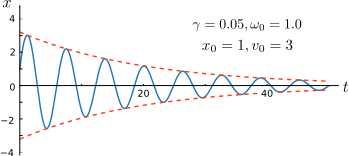
\includegraphics[width=0.61\textwidth]{underdamped}
\end{figure}

\subsubsection{Over-damped motion}
\label{overdamped}

For $\omega_0 < \gamma$, the square root term is imaginary. It is
convenient to define
\begin{equation}
\Gamma = \sqrt{\gamma^2 - \omega_0^2} \quad \Rightarrow \quad \sqrt{\omega_0^2 - \gamma^2} = i \Gamma.
\end{equation}
Then the real solution simplifies in a different way:
\begin{align}
  x(t) = \mathrm{Re}\left[z(t)\right]
  &= \mathrm{Re}\left[\psi_+ e^{\left(-\gamma  + \Gamma\right)t} + \psi_- e^{\left(-\gamma - \Gamma\right)t} \right] \\
  &= C_+ e^{-(\gamma - \Gamma) t} + C_- e^{-(\gamma + \Gamma) t},
  \label{overdamped-sol}
\end{align}
where
\begin{equation}
C_\pm = \mathrm{Re}[\psi_\pm].
\end{equation}
This is called an \textbf{over-damped solution}.  It consists of two
terms, both exponentially decaying in time, with $(\gamma-\Gamma)$ and
$(\gamma + \Gamma)$ serving as the decay rates. Note that both decay
rates are positive real numbers, because $\Gamma < \gamma$ from the
definition of $\Gamma$.  Also, note that $(\gamma - \Gamma)$
\emph{decreases} with $\gamma$, whereas $(\gamma + \Gamma)$
\emph{increases} with $\gamma$, as shown below:

\begin{figure}[ht]
  \centering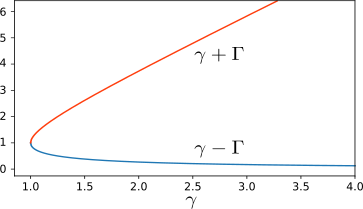
\includegraphics[width=0.55\textwidth]{decay_rates}
\end{figure}

\clearpage
The plot below shows trajectory of the over-damped oscillator:

\begin{figure}[ht]
  \centering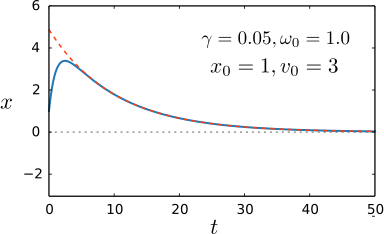
\includegraphics[width=0.5\textwidth]{overdamped}
\end{figure}

\noindent
The red dashes show the limiting curve determined by the decay rate
$(\gamma - \Gamma)$.  The other decay rate, $(\gamma + \Gamma)$,
corresponds to a faster-decaying exponential, so at long times the
second term in Eq.~\eqref{overdamped-sol} becomes negligible compared
to the first term. Then the solution approaches the limit
\begin{equation}
x(t) \approx C_+ e^{-(\gamma - \Gamma) t} \qquad (\mathrm{for}~\mathrm{large}~t).
\label{overdamped-long-t}
\end{equation}
Interestingly, since $(\gamma-\Gamma)$ is a decreasing function of
$\gamma$, \emph{the stronger the damping, the slower the decay rate at
  long times}. This is the opposite of what happens in the
under-damped regime!

Why does this happen? In the over-damped regime, the motion of the
oscillator is dominated by the damping force rather than the spring
force; as the oscillator tries to return to its equilibrium position
$x = 0$, the damping acts against this motion. Hence, the stronger the
damping, the slower the decay to equilibrium. This contrasts sharply
with the Section \ref{underdamped}, where the spring force dominates the
damping force. In that case, stronger damping speeds up the decay to
equilibrium, by causing the kinetic energy of the oscillation to
dissipate more rapidly.

\subsubsection{Critical damping}
\label{critical-damping}

\textbf{Critical damping} occurs when $\omega_0 = \gamma$. Under this
special condition, Eq.~\eqref{gensol} reduces to
\begin{equation}
z(t) = \left(\psi_+ + \psi_-\right) e^{-\gamma t}.
\end{equation}
This has only \emph{one} independent complex parameter, i.e.~the
parameter $(\psi_+ + \psi_-)$. Therefore, it cannot be a general
solution for the complex damped harmonic oscillator equation, which is
still a second-order ODE.

We will not go into detail here regarding the procedure for finding the
general solution for the critically-damped oscillator, leaving it as an
Section \ref{exercises} for the interested reader. Basically, the
procedure is to Taylor expand the solution on either side of the
critical point, and then show that there is a solution of the form
\begin{equation}
z(t) = \left(A + B t\right)\, e^{-\gamma t},
\label{critical-sol}
\end{equation}
which contains the desired two independent parameters.

The critically-damped solution contains an exponential decay constant
of $\gamma$, which is the same as the decay constant for the envelope
function in the under-damped regime [Eq.~\eqref{underdamped-sol}], and
\emph{smaller} than the long-time decay constants in the over-damped
regime [Eq.~\eqref{overdamped-long-t}]. Hence, we can regard the
critically-damped solution as the \emph{fastest-decaying
  non-oscillatory solution}.

This feature of critical damping is employed in many engineering
contexts, the most familiar being automatic door closers. If the
damping is too weak or the spring force is too strong (under-damped),
the door will slam shut, whereas if the damping is too strong or the
spring force is too weak (under-damping), the door takes unnecessarily
long to close. Hence, door closers must be tuned to a ``sweet spot''
corresponding to the critical damping point.

\subsection{Stating the solution in terms of initial conditions}
\label{stating-the-solution-in-terms-of-initial-conditions}

The general solution for the complex damped harmonic oscillator
equation, Eq.~\eqref{gensol}, contains two undetermined parameters
which are the complex amplitudes of the ``clockwise'' and
``counterclockwise'' complex oscillations:
\begin{equation}
z(t) = \psi_+ e^{-i\omega_+ t} + \psi_- e^{-i\omega_- t}, \quad\mathrm{where} \;\; \omega_\pm =  -i\gamma  \pm \sqrt{\omega_0^2 - \gamma^2}.
\end{equation}
However, mechanics problems are often expressed in terms of an
\textbf{initial value problem}, specifying the state of the system at
some initial time $t = 0$. In other words, given $z(0) \equiv x_0$
and $\dot{z}(0) \equiv v_0$, what is $z(t)$ in terms of $x_0$ and
$v_0$?

We can solve the initial-value problem by finding $z(0)$ and
$\dot{z}(0)$ in terms of the above general solution for $z(t)$. The
results are
\begin{align}
  z(0) &= \quad \psi_+ + \psi_- &= x_0& \\
  \dot{z}(0) &= -i\omega_+ \psi_+ - i \omega_- \psi_- &= v_0&.
\end{align}
These two equations can be combined into a 2x2 matrix equation:
\begin{equation}
\begin{bmatrix}1 & 1 \\ -i\omega_+ & -i\omega_-\end{bmatrix} \begin{bmatrix}\psi_+ \\ \psi_-\end{bmatrix} = \begin{bmatrix}x_0 \\ v_0\end{bmatrix}.
\end{equation}
So long as the system is not at the critical point (i.e.,
$\omega_+ \ne \omega_-$), the matrix is non-singular, and we can
invert it to obtain $\psi_\pm$:
\begin{equation}
\begin{bmatrix}\psi_+ \\ \psi_-\end{bmatrix} = \frac{1}{i(\omega_+-\omega_-)}\begin{bmatrix}-i\omega_-x_0 - v_0 \\ i\omega_+x_0 + v_0 \end{bmatrix}.
\end{equation}
We can plug these coefficients back into the general solution. After
some algebra, the result simplifies to
\begin{equation}
z(t) = e^{-\gamma t} \left[x_0 \cos(\Omega t) + \frac{\gamma x_0 + v_0}{\Omega} \, \sin(\Omega t)\right], \;\; \mathrm{where}\;\; \Omega \equiv \sqrt{\omega_0^2 - \gamma^2}.
\end{equation}
For the under-damped case, $\Omega$ is real, and this solution is
consistent with the one found in Section~\ref{underdamped}, except
that it is now explicitly expressed in terms our initial conditions
$x_0$ and $v_0$.  As for the over-damped case, we can perform the
replacement
\begin{equation}
\Omega \rightarrow i \Gamma = i \sqrt{\gamma^2 - \omega_0^2}.
\end{equation}
Then, using the relationships between trigonometric and hyperbolic
functions discussed in Section 3.5.3, the solution can be re-written
as
\begin{align}
  z(t) &= e^{-\gamma t} \left[x_0 \cosh(\Gamma t) + \frac{\gamma x_0 + v_0}{i\Gamma} \, i \sinh(\Gamma t)\right] \\
  &= \left(\frac{x_0}{2} + \frac{\gamma x_0 + v_0}{2\Gamma}\right) e^{-(\gamma - \Gamma) t} + \left(\frac{x_0}{2} - \frac{\gamma x_0 + v_0}{2\Gamma}\right) e^{-(\gamma+\Gamma)t},
\end{align}
which is consistent with the solution found in
Section~\ref{overdamped}.

In either case, so long as we plug in real values for $x_0$ and $v_0$,
the solution is guaranteed to be real for all $t$. That's to be
expected, since the real solution is also one of the specific
solutions for the complex harmonic oscillator equation.

\subsection{Exercises}
\label{exercises}

\begin{enumerate}
\item
  In Section~\ref{complex-frequencies}, we encountered the complex
  frequencies
  \begin{equation}
    \omega_\pm = -i\gamma \pm \sqrt{\omega_0^2 - \gamma^2}.
  \end{equation}
  For fixed $\omega_0$ and $\omega_0 > \gamma$ (under-damping), prove
  that $\omega_\pm$ lie along a circular arc in the complex plane.

\item
  Derive the general solution for the critically damped harmonic
  oscillator, Eq.~\eqref{critical-sol}, by following these steps:
  \begin{enumerate}[(a)]
  \item
    Consider the complex ODE, in the under-damped regime $\omega_0 >
    \gamma$. We saw in Section~\ref{general-solution} that the general
    solution has the form
    \begin{equation}
      z(t) = \psi_+ \, \exp\left[\left(-\gamma  - i \sqrt{\omega_0^2 - \gamma^2}\right)t\right] \; +\; \psi_- \, \exp\left[\left(-\gamma +i\sqrt{\omega_0^2 - \gamma^2}\right)t\right]
    \end{equation}
    for some complex parameters $\psi_+$ and $\psi_-$. Define the
    positive parameter $\varepsilon = \sqrt{\omega_0^2 - \gamma^2}$.
    Re-write $z(t)$ in terms of $\gamma$ and $\varepsilon$ (i.e.,
    eliminating $\omega_0$).

  \item
    The expression for $z(t)$ is presently parameterized by the
    independent parameters $\psi_+$, $\psi_-$, $\varepsilon$, and
    $\gamma$. We are free to re-define the parameters, by taking
    \begin{align}
      \alpha &= \psi_+ + \psi_- \\
      \beta &= -i\varepsilon(\psi_+ - \psi_-).
    \end{align}
    Using these equations, express $z(t)$ using a new set of
    independent complex parameters, one of which is $\varepsilon$.
    Explicitly identify the other independent parameters, and state
    whether they are real or complex.
  \item
    Expand the exponentials in $z(t)$ in terms of the parameter
    $\varepsilon$. Then show that in the limit $\varepsilon
    \rightarrow 0$, $z(t)$ reduces to the critically-damped general
    solution \eqref{critical-sol}.
  \end{enumerate}

\item
  Repeat the above derivation for the critically-damped solution, but
  starting from the over-damped regime $\gamma > \omega_0$.

\item
  Let $z(t)$ be a complex function of a real input $t$, which obeys
  the differential equation
  \begin{equation}
    \frac{dz}{dt} = -i\,(\omega_1 - i \gamma)\; z(t),
  \end{equation}
  where $\omega_1$ and $\gamma$ are real. Find the general solution
  for $z(t)$, and hence show that $z(t)$ satisfies the damped
  oscillator equation
  \begin{equation}
    \left[\frac{d^2}{dt^2} + 2\gamma \frac{d}{dt} + \omega_0^2 \right] z(t) = 0
  \end{equation}
  for some $\omega_0^2$. Finally, show that this harmonic oscillator
  is always under-damped.
\end{enumerate}


\end{document}
